\documentclass[notes,11pt, aspectratio=169]{beamer}
\usetheme{default}
\usepackage{helvet}
\usepackage[default]{lato}
\usepackage{amsmath}
\usepackage{mathpazo}
\usepackage{hyperref}
\usepackage{lipsum}
\usepackage{multimedia}
\usepackage{graphicx}
\usepackage{multirow}
\usepackage{graphicx}
\usepackage{changepage}
\usepackage{booktabs}
\usepackage{appendixnumberbeamer}

\usepackage{tabularray}
\usepackage{float}
\usepackage{codehigh}
\usepackage[normalem]{ulem}
\UseTblrLibrary{siunitx}
\newcommand{\tinytableTabularrayUnderline}[1]{\underline{#1}}
\newcommand{\tinytableTabularrayStrikeout}[1]{\sout{#1}}
\NewTableCommand{\tinytableDefineColor}[3]{\definecolor{#1}{#2}{#3}}



\newcommand{\beginbackup}{
   \newcounter{framenumbervorappendix}
   \setcounter{framenumbervorappendix}{\value{framenumber}}
   \setbeamertemplate{footline}
   {
     \leavevmode%
     \hline
     box{%
       \begin{beamercolorbox}[wd=\paperwidth,ht=2.25ex,dp=1ex,right]{footlinecolor}%
%         \insertframenumber  \hspace*{2ex}
       \end{beamercolorbox}}%
     \vskip0pt%
   }
 }
\newcommand{\backupend}{
   \addtocounter{framenumbervorappendix}{-\value{framenumber}}
   \addtocounter{framenumber}{\value{framenumbervorappendix}}
}
% These are my colors -- there are many like them, but these ones are mine.
\definecolor{blue}{RGB}{0,114,178}
\definecolor{red}{RGB}{213,94,0}
\definecolor{yellow}{RGB}{240,228,66}
\definecolor{green}{RGB}{0,158,115}

\hypersetup{
  colorlinks=false,
  linkbordercolor = {white},
  linkcolor = {blue}
}


%% I use a beige off white for my background
\definecolor{MyBackground}{RGB}{255,253,218}
\setbeamercolor{frametitle}{fg=blue}
\setbeamercolor{title}{fg=black}
\setbeamertemplate{footline}[frame number]
\setbeamertemplate{navigation symbols}{}
\setbeamertemplate{itemize items}{-}
\setbeamercolor{itemize item}{fg=blue}
\setbeamercolor{itemize subitem}{fg=blue}
\setbeamercolor{enumerate item}{fg=blue}
\setbeamercolor{enumerate subitem}{fg=blue}
\setbeamercolor{button}{bg=MyBackground,fg=blue,}
\setbeamercolor{section in toc}{fg=blue}
\setbeamercolor{subsection in toc}{fg=red}
\setbeamersize{text margin left=1em,text margin right=1em}

\newenvironment{wideitemize}{\itemize\addtolength{\itemsep}{10pt}}{\enditemize}

% Customizing footer to display only the current page number
% Customizing footer: Right-aligned but with some padding from the edge
\setbeamertemplate{footline}{%
  \hfill
  \begin{beamercolorbox}[wd=\paperwidth,ht=0.4cm,dp=0.3cm,right]{footline}%
    \hspace{-1cm} \insertframenumber\hspace{0.2cm} % Adjust the spacing here
  \end{beamercolorbox}%
}

\title{\textcolor{blue}{Immigration and armed conflicts: Era of globalization}}

\author{Hyoungchul Kim}

\institute{Wharton UPenn}

\date{\today}

\begin{document}

\begin{frame}[plain]
	\titlepage
\end{frame}

\setcounter{framenumber}{0}

\begin{frame}{Recap: Food for thought}
	\textbf{Will immigration increase/decrease conflicts?} \textcolor{red}{Not easy to answer.}	
	\begin{itemize}
		\item \textbf{Increase}: (1) Conflicts between natives (2) Bring immigrants' conflicts into the country.  
		\item \textbf{Decrease}: Higher proportion of immigration may increase the opportunity cost for one group to disturb the peace.
	\end{itemize}\vspace{1em}

	\textbf{Indirect effect could also matter!}
	\begin{itemize}
		\item The opportunity cost of starting a war could increase if the opponent has large portion of immigration from other countries.
	\end{itemize}
\end{frame}

\begin{frame}{Recap: Research question}
	\textbf{Does immigration increase or decrease war/armed conflicts?}	
	\begin{itemize}
		\item Heterogeneous effects depending on the types of conflict.
		\item Direct and indirect effect of immigration.
	\end{itemize}\vspace{1em}

	\textbf{Research design}
	\begin{itemize}
		\item Use worldwide immigration patterns from 1990-2022.
		\item Identification strategy: Shift-share IV to causally estimate the impact of immigration.
	\end{itemize}
\end{frame}

\begin{frame}{(Updated) Preview of results}
	\textbf{Some trial and error}
	\begin{itemize}
		\item Applied shift-share IV regression to estimate impact of immigration on intrastate conflict.
		\item Regression specification not robust to the change in specification.
		\item \textcolor{red}{\textbf{Dig into the descriptive statistics of the main outcome (intra- interstate war) to check any patterns in the data.}}
		\item Try out different specification for IV.
		\item Pivot? \textcolor{red}{\textbf{Different data?}}
	\end{itemize}
\end{frame}

\begin{frame}{(Recap) Data}
	\textbf{Immigration}
	\begin{itemize}
		\item UN Global migration database (1990-2024, 5 years): Destination-origin pair of immigration stock, at least 190 countries every year. 
		\item World Bank migration data (1960-2000, decennial): Use it for exogenous IV share.
	\end{itemize}\vspace{1em}

	\textbf{Armed conflicts}
	\begin{itemize}
		\item UCDP/PRIO Armed conflict dataset (1946-2022, annually): Incidence of conflicts (at least 25 battle death, interstate, intrastate) 
	\end{itemize}\vspace{1em}

	\textbf{Other data for controls}
	\begin{itemize}
		\item CEPII: Trade volume, GDP, WTO, GATT, etc.
	\end{itemize}\vspace{1em}
	\begin{center}
	\textbf{Final sample: 1990-2022, destination-origin pair of countries}.
	\end{center}
\end{frame}

\begin{frame}{Summary statistics: Conflicts data}
\begin{columns}
\begin{column}{0.5\textwidth}
\begin{figure}
	\centering
	\resizebox{0.4\textwidth}{!}{
		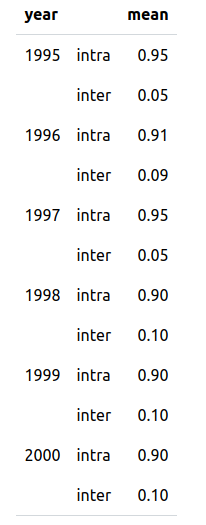
\includegraphics{conft.png}
	}
\end{figure}	
\end{column}
\begin{column}{0.5\textwidth}
	\begin{wideitemize}
	\item \textbf{(mean)} should be understood as proportions here.
	\item Most of the conflicts are intrastate.
	\item Unlike interstate, there can be other various factors leading to intrastate conflicts, lessening the effect from immigrant. 
	\end{wideitemize}	
\end{column}
\end{columns}
\end{frame}

\begin{frame}{Conflicts data visualization: Intrastate}
\begin{figure}
	\centering
	\resizebox{0.75\textwidth}{!}{
		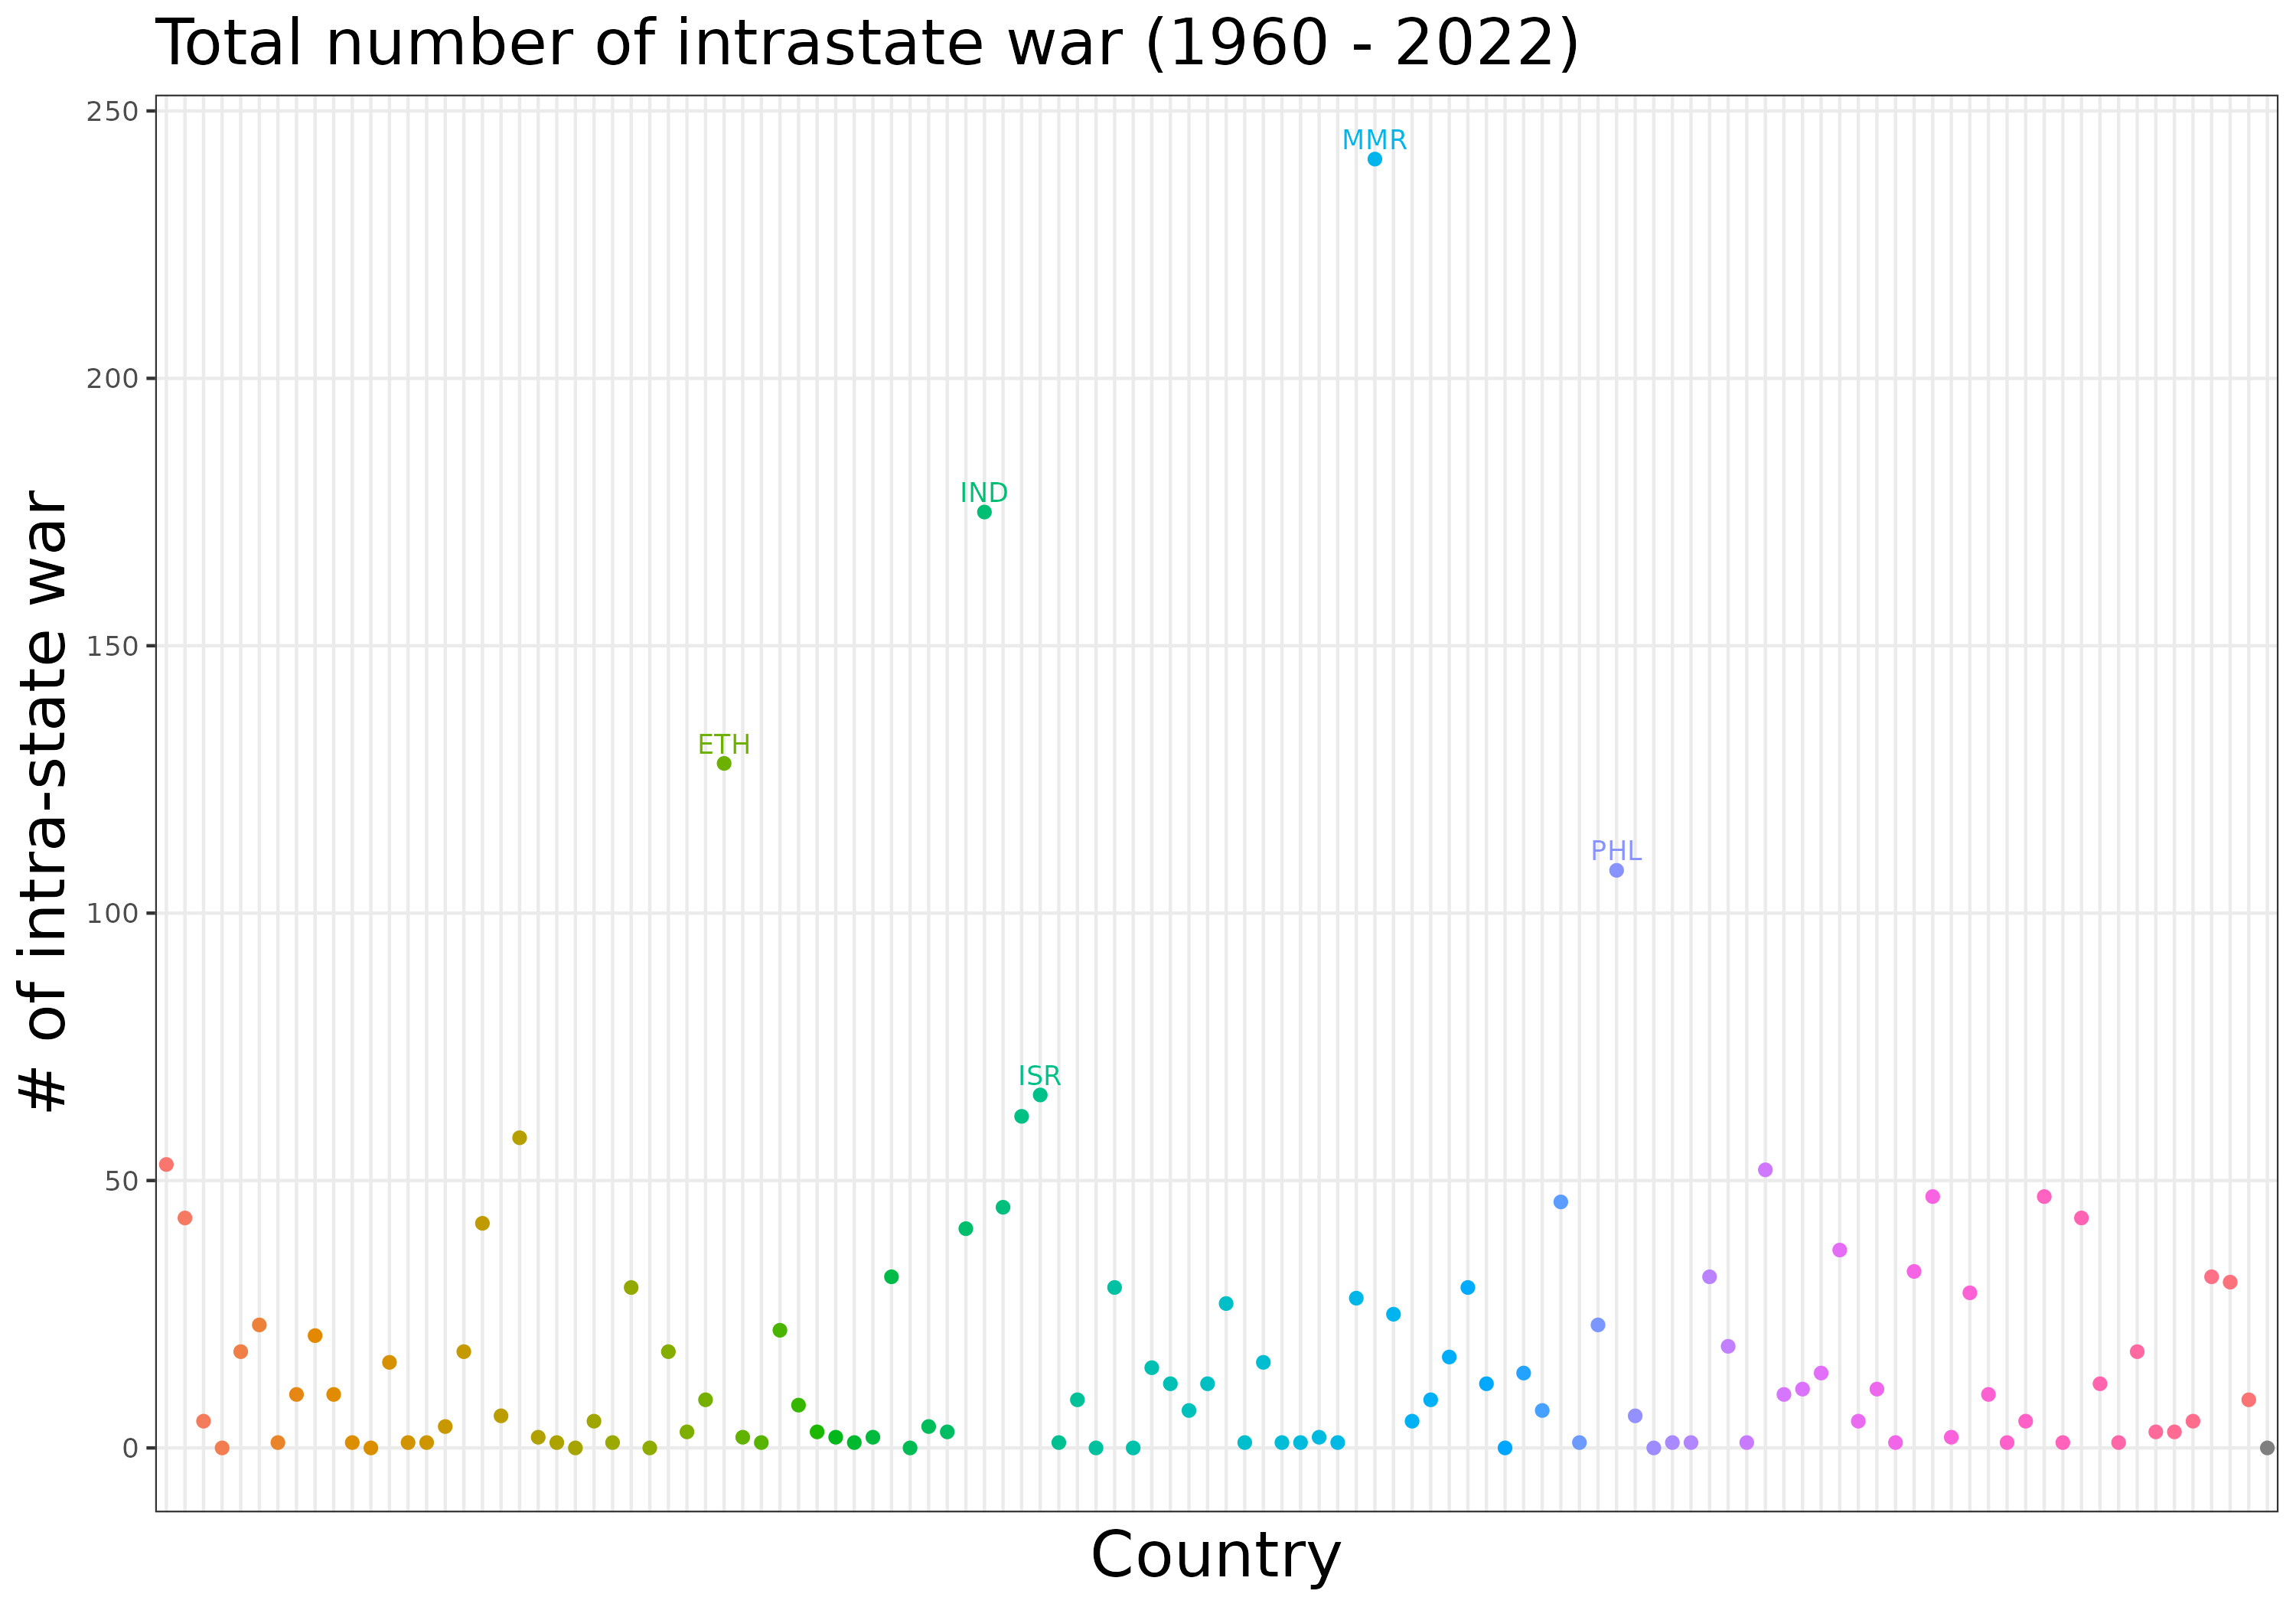
\includegraphics{intra.png}
	}
\end{figure}	
\end{frame}

\begin{frame}{Conflicts data visualization: Interstate}
	
\begin{figure}
	\centering
	\resizebox{0.75\textwidth}{!}{
		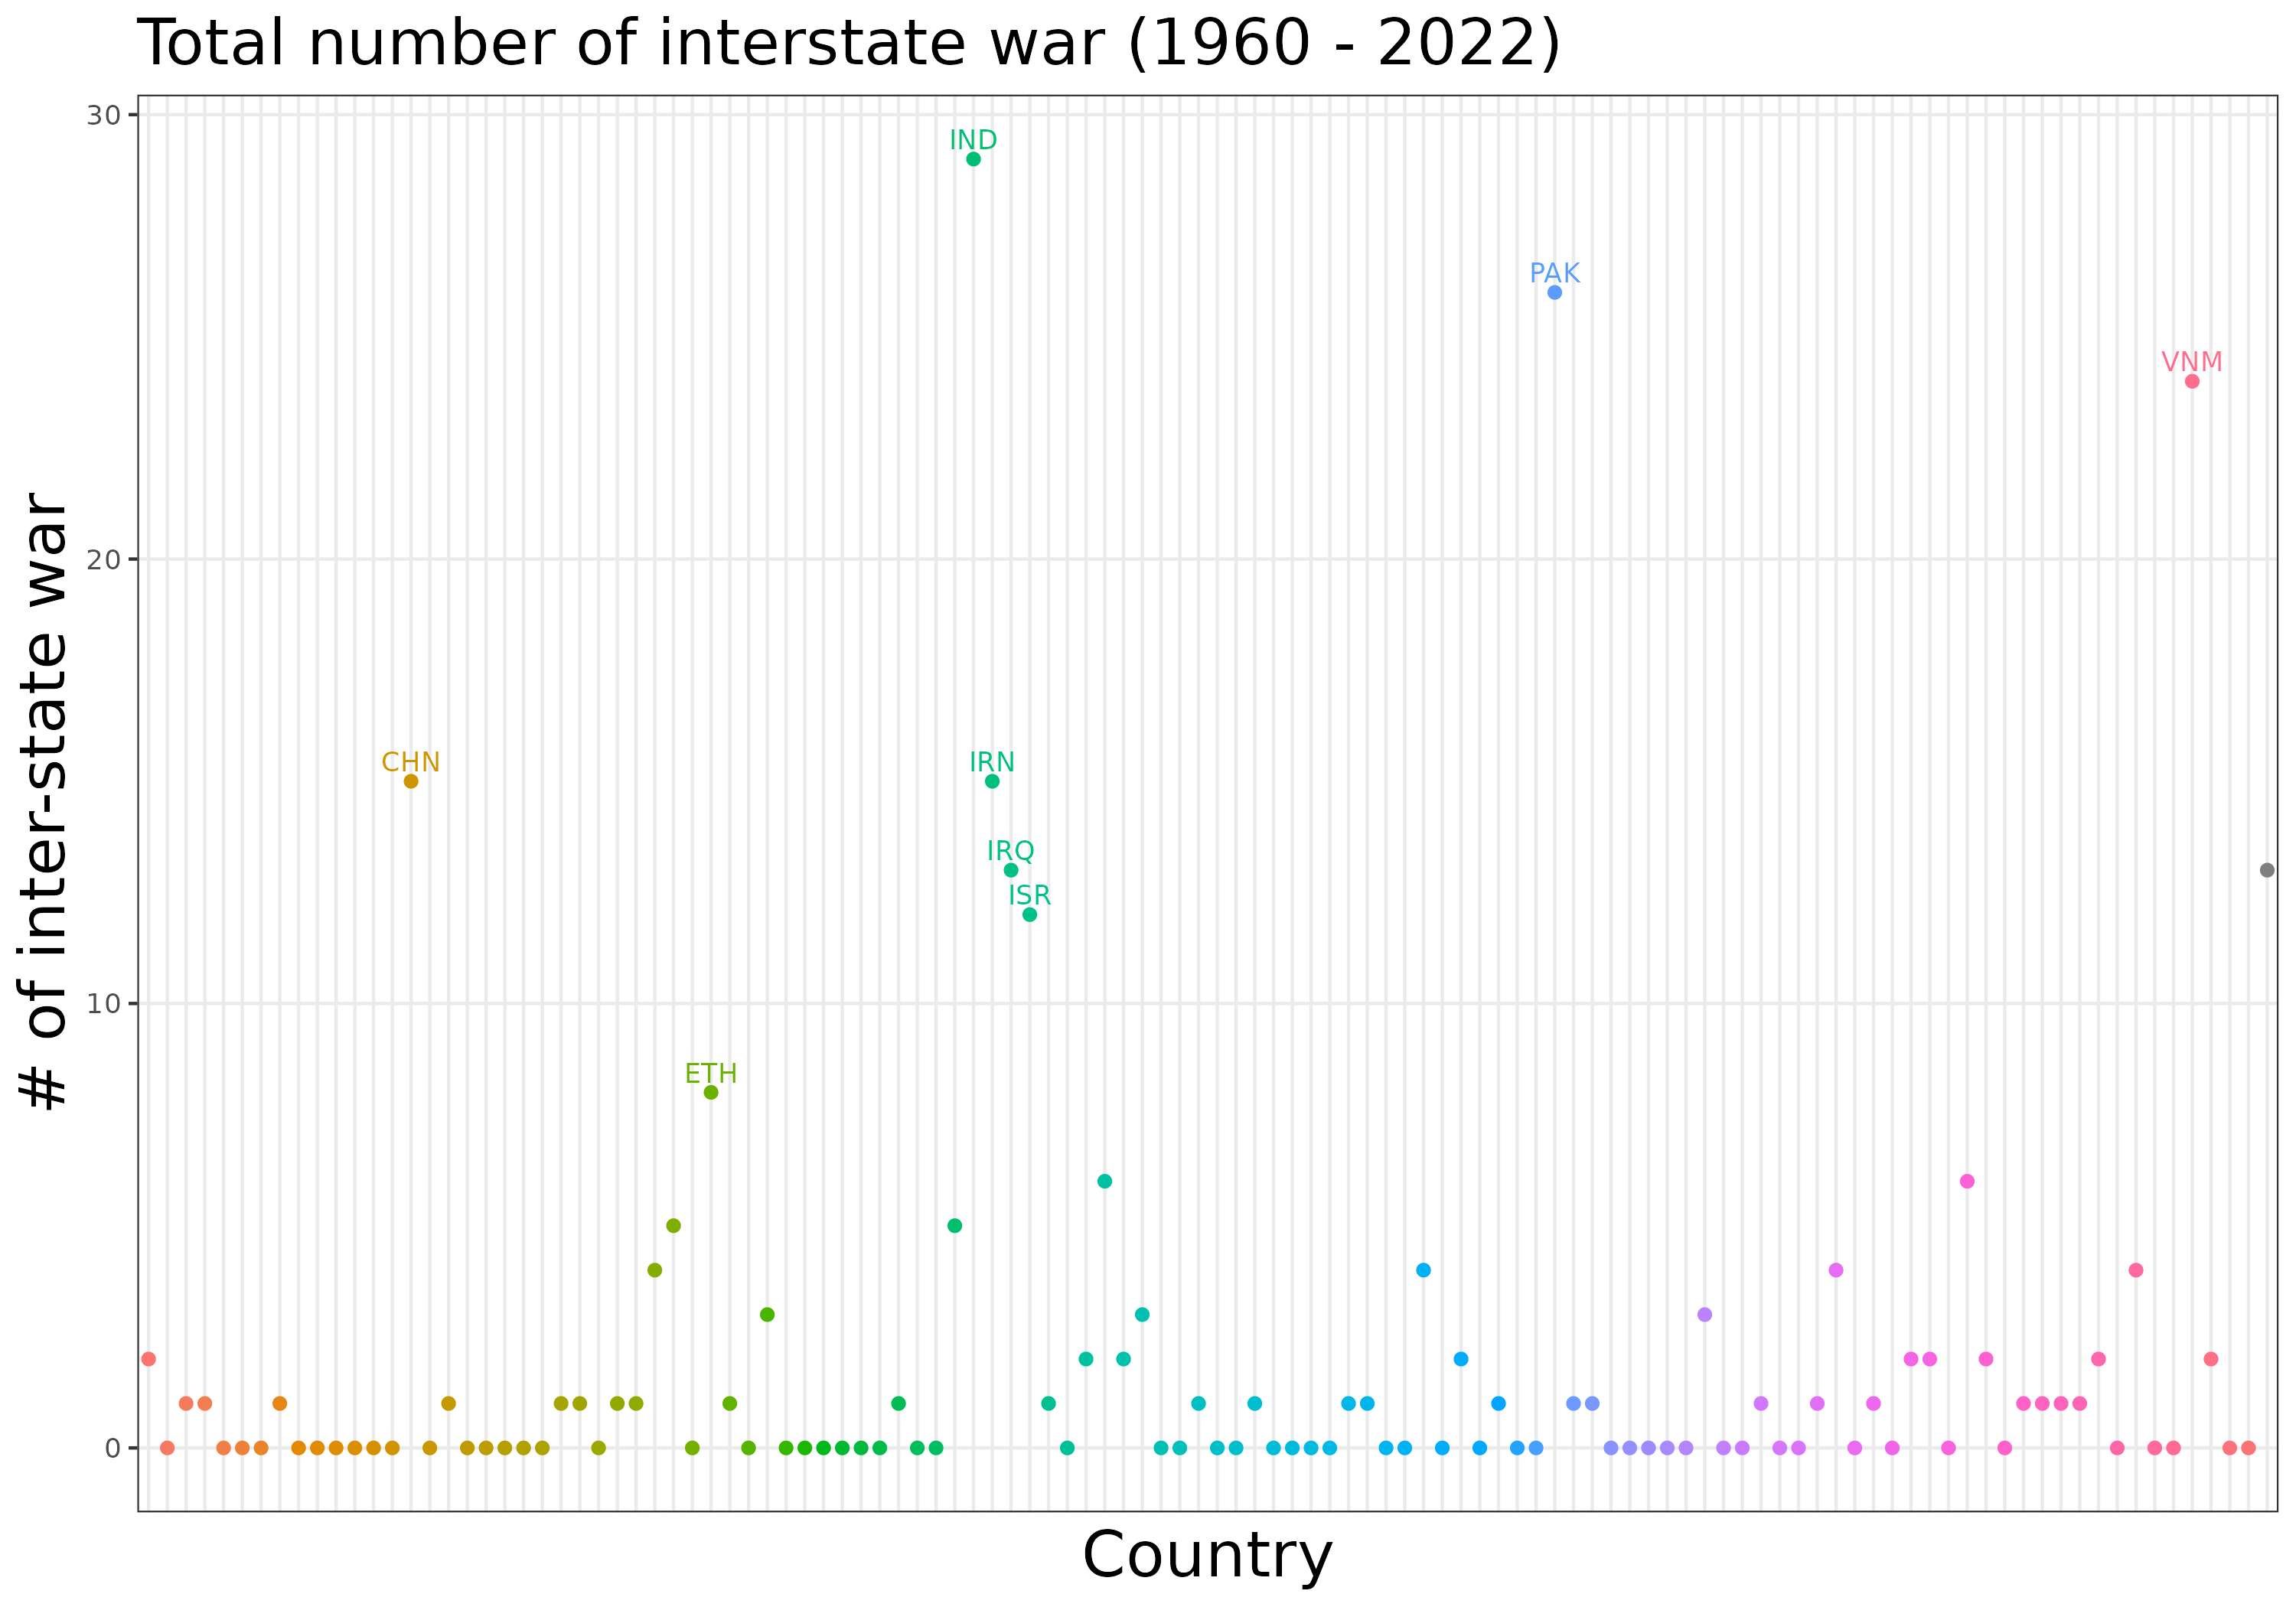
\includegraphics{inter.png}
	}
\end{figure}	
\end{frame}

\begin{frame}{Summary statistics: Immigrant data}
\begin{table}
	\centering
	\begin{tabular}{lrr}
		\toprule
		year & immigration stock (total) & immigration share (mean) \\
		\midrule
		1960 & 71,124,984 & 0.055\\
		1970 & 80,422,844 & 0.069\\
		1980 & 92,427,478 & 0.074\\
		\midrule
		1990 & 139,297,313 & 0.088\\
		2000 & 163,748,711 & 0.093\\
		\bottomrule
	\end{tabular}
\end{table}	
\begin{wideitemize}
\item Noticeable jump from 1980 to 1990.
\item Is this data issue? Or is this some true exogenous shock (immigration policy change, globalization, etc).
\end{wideitemize}
\end{frame}

\begin{frame}{Immigration data visualization}
\begin{figure}
	\centering
	\resizebox{0.75\textwidth}{!}{
		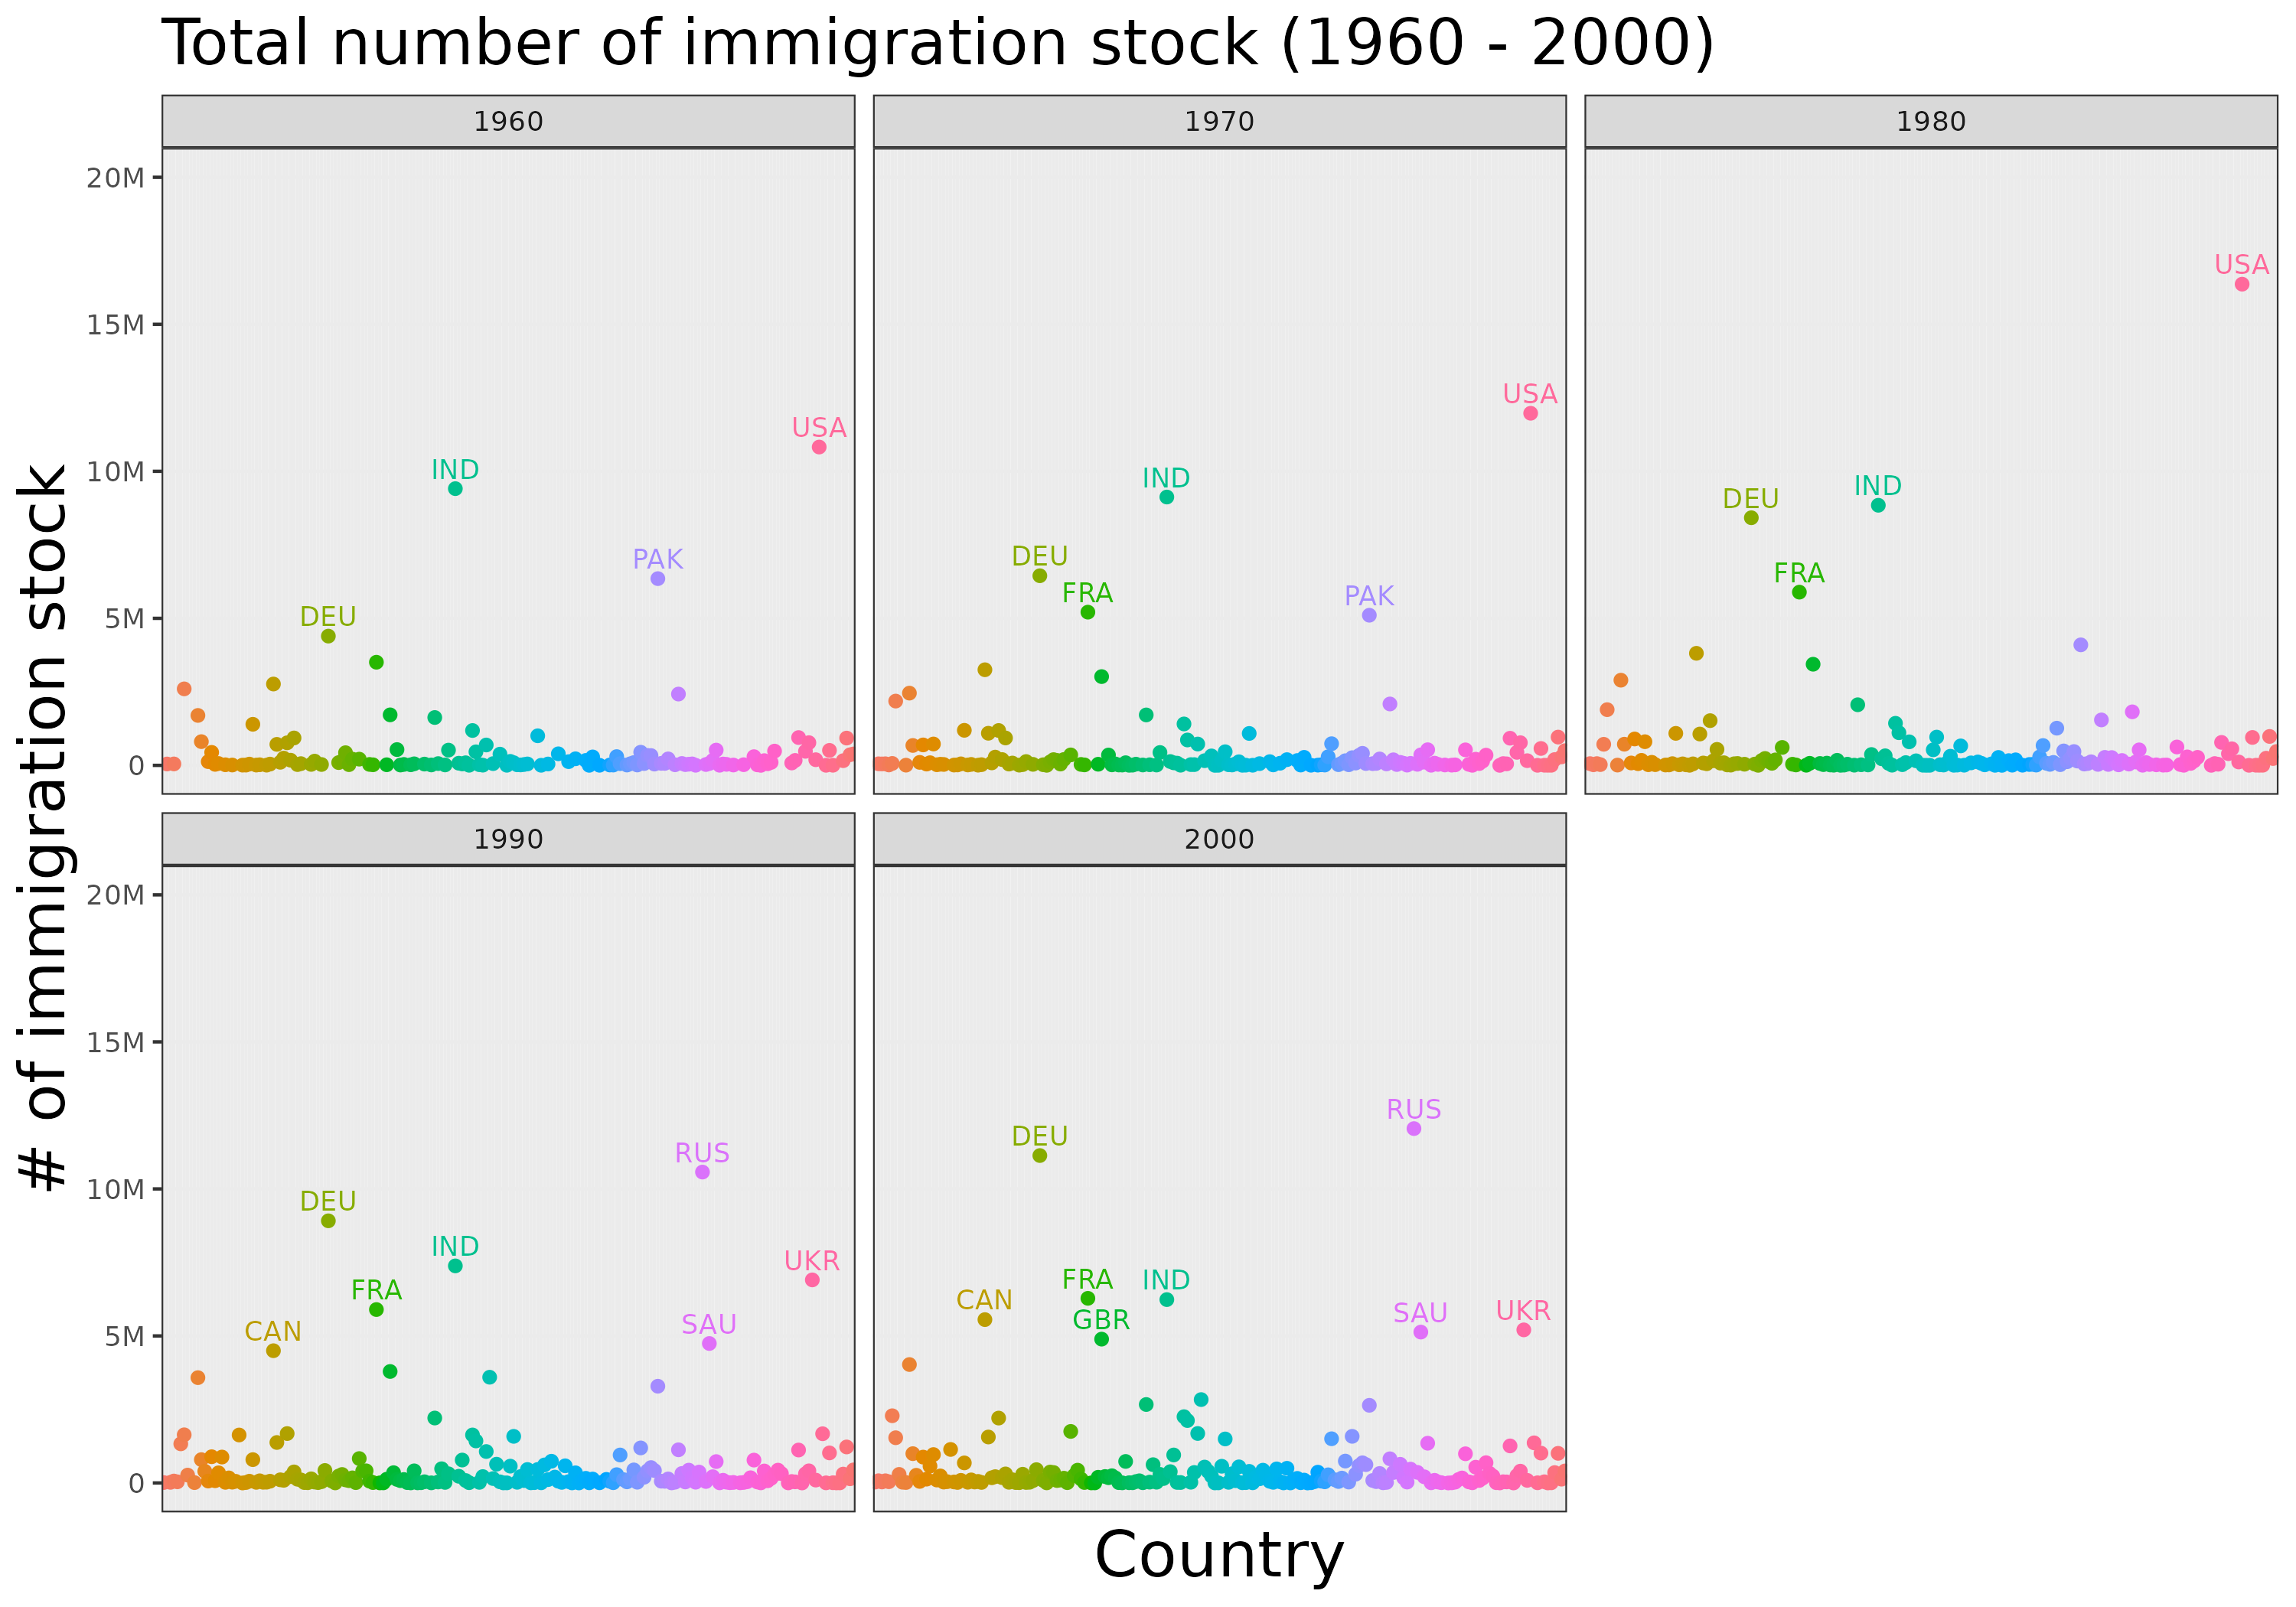
\includegraphics{imm.png}
	}
\end{figure}	
\end{frame}

\begin{frame}{Baseline regression}
	We aggregate the destination-origin pair to destination for now.
\begin{align*}
	y_{it} = \alpha + \beta D_{it} + \Gamma' X_{it} + \varepsilon_{it}. 
\end{align*}	

\begin{itemize}
	\item Note that the years are aggregated to every 5 years.
	\item $y_{it}$ is the cumulative sum of conflicts that country $i$ was involved in during 5 years after year $t$.
	\item $D_{it}$ is share of share of total immigration stock (w.r.t. total population) in start of the year $T$. 
\end{itemize}
\end{frame}


\begin{frame}{Identification strategy: Shift-share IV}
	We construct shift-share IV as follows:
	\begin{align*}
		D_{it} &= \text{IMM}_{it} / \text{POP}_{it} \quad \text{where}\\ \nonumber  
		\text{IMM}_{it}  &= \widehat{\text{IMM}_{i,t-1}} +  \sum_j \overbrace{\text{WORLD}_{j,t-1}}^{\textcolor{red}{\text{Shift}}} \times \underbrace{\frac{\text{CNTRY}_{ij, 1960}}{\text{CNTRY}_{i,1960}}}_{\textcolor{red}{\text{Share}}}	
	\end{align*}

	\begin{itemize}
		\item $\text{IMM}_{it}$ is number of immigration stock in country $i$ in year $t$.
		\item $\text{WORLD}_{j,t-1}$ is the number of total immigration flow  coming out from country $j$ between year $t$ and $t-1$.
		\item $\text{CNTRY}$ just implies the share of immigration stock in country $i$ that came from country $j$ in year 1960.
		\item Identification assumption: (1) Some exogenous portion of immigration shift starting from 1990s, (2) Some exogenous portion of immigration share by fixing it to 1960.
	\end{itemize}
\end{frame}

\begin{frame}{First-stage result}
	\begin{figure}
		\resizebox{\textwidth}{!}{
		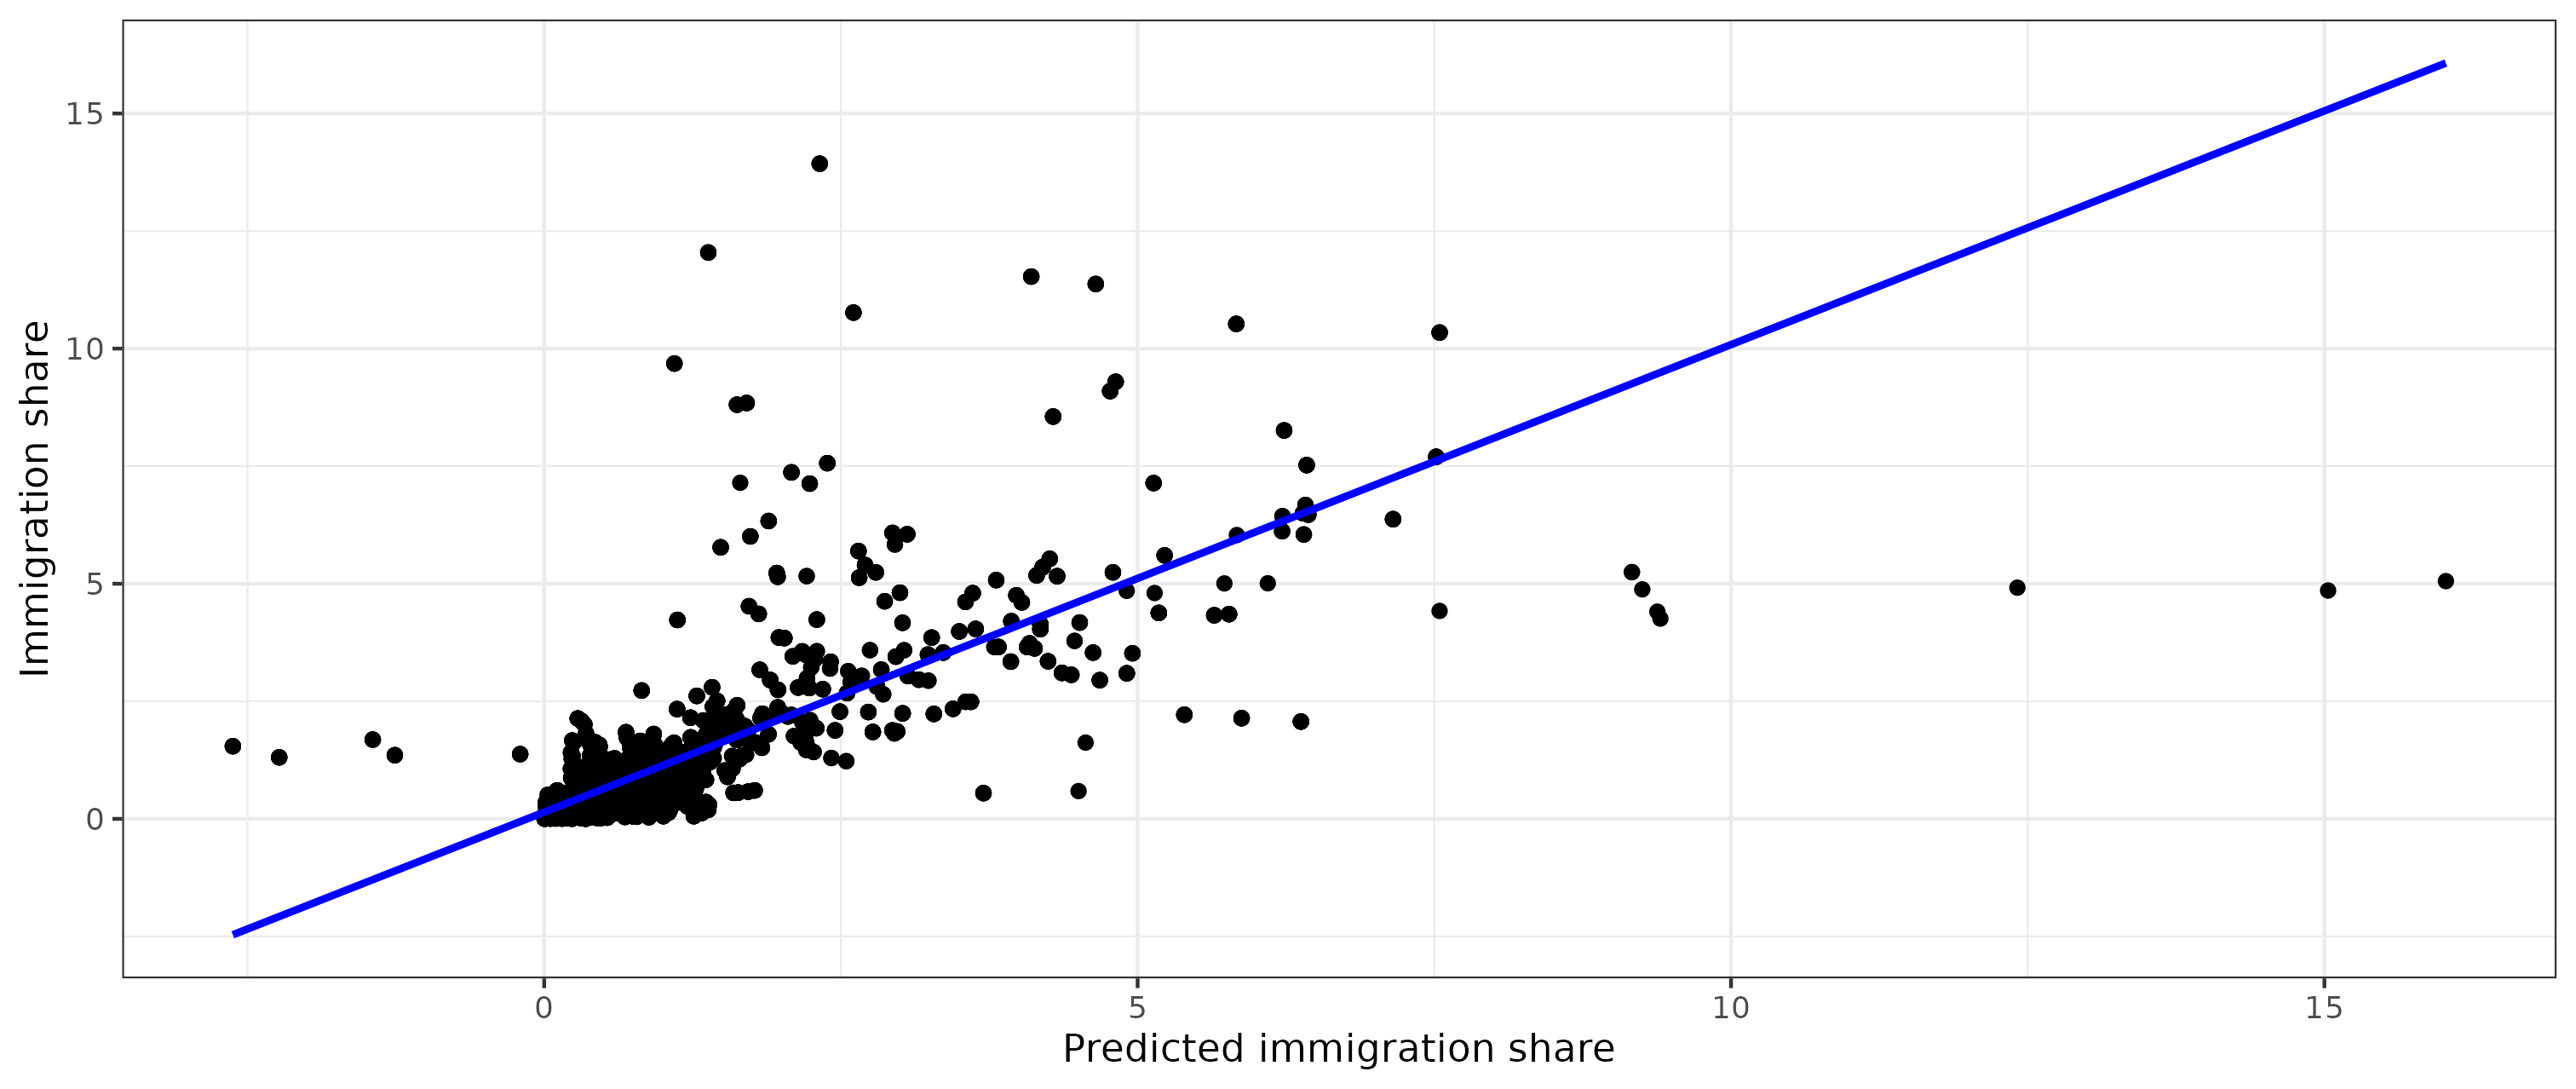
\includegraphics{first.png}}
	\end{figure}	
	IV's predictive power seems to be pretty great but values are kinda weird$\ldots$ Perhaps due to some measurement error (or my error).
\end{frame}

\begin{frame}{2SLS results}
\begin{table}
	\resizebox{0.8\textwidth}{!}{
	
\begingroup
\centering
\begin{tabular}{lccccc}
   \toprule
    & \multicolumn{5}{c}{\# Intrastate conflict}\\
                     & (1)                     & (2)          & (3)          & (4)                 & (5)\\  
   \midrule 
   Immigration Share & -0.00029163$^{***}$     & -0.00029052  & -0.00029163  & 0.00041893$^{**}$   & 0.00041893\\   
                     & ($5.38\times 10^{-5}$)  & (0.00023524) & (0.00019798) & (0.00016932)        & (0.00056018)\\   
   log(flow)         &                         &              &              & -0.06130469$^{***}$ & -0.06130469\\   
                     &                         &              &              & (0.01799096)        & (0.05732256)\\   
   log(pop)          &                         &              &              & 1.100261$^{***}$    & 1.100261$^{**}$\\   
                     &                         &              &              & (0.12846441)        & (0.43693673)\\   
   log(gdp)          &                         &              &              & -0.62370974$^{***}$ & -0.62370974$^{**}$\\   
                     &                         &              &              & (0.09568586)        & (0.31618421)\\   
   gatt              &                         &              &              & 1.046485$^{***}$    & 1.046485$^{**}$\\   
                     &                         &              &              & (0.11188113)        & (0.44104420)\\   
   wto               &                         &              &              & -1.667242$^{***}$   & -1.667242$^{***}$\\   
                     &                         &              &              & (0.15164586)        & (0.41570825)\\   
   \midrule 
   year FE           &                         &              &              & Yes                 & Yes\\  
   region FE         &                         &              &              & Yes                 & Yes\\  
   \midrule 
   Observations      & 5,038                   & 5,027        & 5,038        & 4,902               & 4,902\\  
   R$^2$             & 0.02158                 & 0.02164      & 0.02158      & 0.19674             & 0.19674\\  
   F-stage           & 57.2                    & 4.462        & 8.997        & 22.1                & 2.29\\  
   \bottomrule
   \multicolumn{6}{l}{\emph{  }}\\
\end{tabular}
\par\endgroup


}
\end{table}	
\begin{footnotesize}
	\textbf{Notes.} ***: 0.01, **: 0.05, *: 0.01
\end{footnotesize}
\end{frame}

\begin{frame}{Alternative Shift-share IV: In progress}

	\begin{wideitemize}
	\item Shift: Total number of immigrants in each period by origin country.
	\item Share: 1960 Share of immigrants in each country by origin country.
	\item Validity: Exogenous shift? Exogenous share?
	\item In fact, I tried this sometime ago: First-stage not strong.
	\end{wideitemize}
	
\end{frame}

\begin{frame}{Discussion: Other data on conflicts?}
	\begin{wideitemize}
	\item There are other data on worldwide conflicts that we can use.
	\item e.g. Correlates of War.
	\item Timespan: 1816 – 2007.
	\item Level of war is higher: At least 1,000 battle death.
	\item Not much info on type of conflict.
	\end{wideitemize}
\end{frame}

\begin{frame}{Discussion: Problems with using two different data on immigration}
	\begin{wideitemize}
	\item In the analysis, I use 1960 immigrant data from World Bank for constructing IV.
	\item But for regressor, I use 1990-2022 immigrant data from UN. 
	\item Since I am using two data for one analysis, this might be problematic (measurement issue).
	\item This could also be the reason why some of my results in first-stage is weird
	\end{wideitemize}	
\end{frame}

\begin{frame}{Conclusion}
\begin{itemize}
	\item Is it an interesting question? $\Rightarrow$ Maybe.
	\item Perhaps relation between immigration and war might not be significant enough.
	\item Better data on immigration? $\Rightarrow$ Not easy to find a better data.
\end{itemize}	
\end{frame}


\end{document}
